\documentclass[dvipsnames]{standalone}
\usepackage[utf8]{inputenc}
\usepackage{tikz}
\usepackage{pgfplots}
\usepackage{pgfkeys}
\usetikzlibrary{
    shadows.blur, 
    arrows, 
    arrows.meta, 
    shapes.arrows, 
    decorations.markings, 
    positioning
}

\pgfplotsset{compat=1.18} 

\colorlet{sp-bg}{SkyBlue!50}
\colorlet{cpu-bg}{LimeGreen!50}
\colorlet{gpu-bg}{Salmon!70}
\colorlet{gpu-mem-bg}{Orchid!50}
\colorlet{host-to-gpu}{RedOrange!60}
\colorlet{gpu-to-host}{CornflowerBlue!80}

\begin{document}

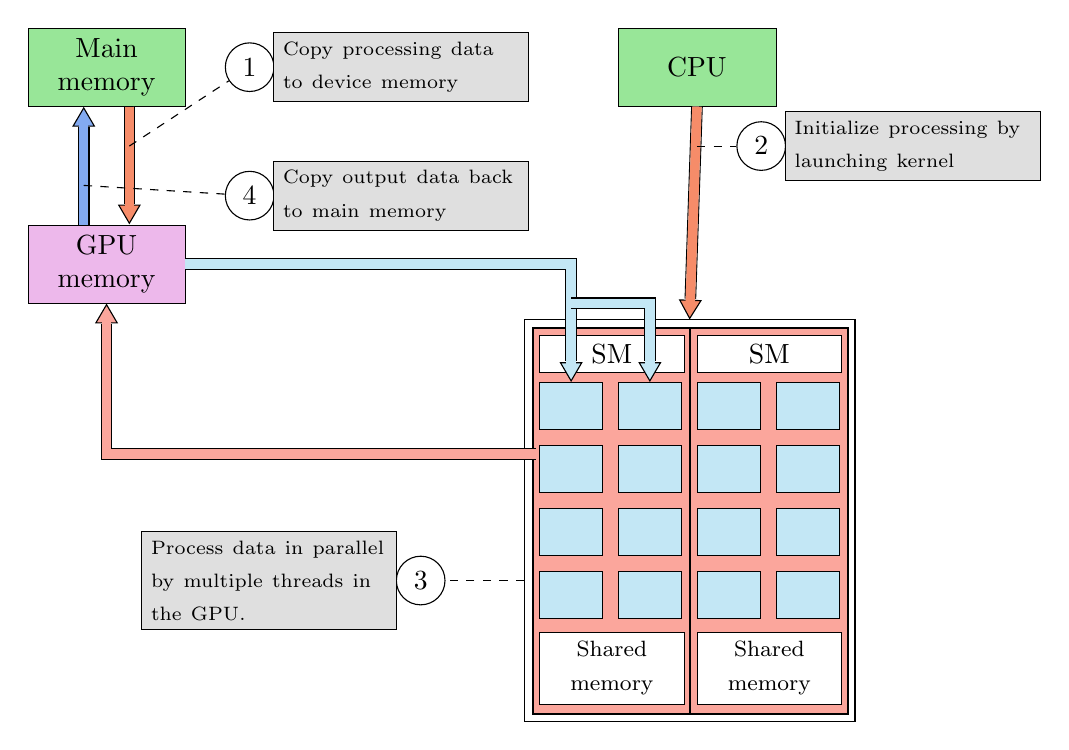
\begin{tikzpicture}[    
    arrow color/.store in=\arrowcolor,
    arrow color=white,
    step pointer/.style={dashed},
    step label/.style={circle,draw},
    step text/.style={
        right=0.3cm,
        draw,
        fill=lightgray!50,
        solid,
        text width=3cm
    },
    vec arrow/.style={        
        thin, 
        decoration={
            markings,            
            mark=at position 1 with {
                \arrow[thin]{Triangle[scale=2,fill=\arrowcolor]}
            }
        },
        double distance=3.4pt, 
        shorten >= 7.5pt,
        preaction = {decorate},
        postaction = {draw,line width=3.4pt,\arrowcolor,shorten >= 4.5pt}
    },
    sp/.style={
        draw=black,
        ultra thin,
        fill=sp-bg,
        minimum width=0.8cm,
        minimum height=0.6cm,
        anchor=north west
    },
    sm bg/.style={
        draw=black,
        thick,
        fill=gpu-bg,
        minimum width=2cm,
        minimum height=4.9cm,
        anchor=north west
    },
    sm label/.style={
        draw=black,
        ultra thin,
        fill=white,
        minimum width=1.8cm,
        align=center,
        text width=1.6cm,
        anchor=north west
    },
    info box/.style={
        minimum width=2cm,
        minimum height=1cm,
        draw=black,
        ultra thin,
        align=center,
        anchor=north west
    },
    sm/.pic={        
        \node[sm bg] (MP) at (-0.1, 3.7) {};
        \foreach \i in {0, 1} {
            \foreach \j in {0, 1, 2, 3} {
                \node[sp] (SP\i\j) at (\i, 0.8*\j+0.6) {};
            }
        }
        \node[sm label] (SM) at (0, 3.6) {SM};
        \node[sm label, below=3.3cm of SM] {\footnotesize Shared memory};
    }
]

\node[info box, fill=cpu-bg, anchor=north] (CPU) at (2, 7.5) {CPU};
\node[info box, fill=cpu-bg] (RAM) at (-6.5, 7.5) {Main\\memory};
\node[info box, fill=gpu-mem-bg] (GPU mem) at (-6.5, 5) {GPU\\memory};

\begin{scope}[local bounding box=GPU]
\node[
    draw=black,
    rectangle, 
    minimum width=4.2cm, 
    minimum height=5.1cm,
    anchor=north west
] at (-0.2, 3.8) {};
\pic (SM1) at (0, 0) {sm};    
\pic (SM2) at (2, 0) {sm};
\end{scope}

\coordinate[above=of SM1SP03.north] (A);

\draw (CPU.south) edge[arrow color=host-to-gpu, vec arrow] (GPU.north);

\draw[to path={-| (\tikztotarget)}]     
    ([xshift=0.05cm]SM1MP.140) edge[arrow color=gpu-bg, vec arrow] (GPU mem.south)
    (GPU mem.east) edge[arrow color=sp-bg, vec arrow] (SM1SP03)
    (GPU mem.120) edge[arrow color=gpu-to-host, vec arrow] (RAM.240)
    (RAM.300) edge[arrow color=host-to-gpu, vec arrow] (GPU mem.60)
    (A) edge[arrow color=sp-bg, vec arrow] (SM1SP13);
;

\coordinate[below=0.5cm of RAM.300] (s1);
\node[right=0.5cm of RAM.east,step label] (l1) {1};
\draw[step pointer] 
    (s1) 
    -- 
    (l1) 
    node[step text] {
        \scriptsize Copy processing data to device memory
    }
;

\coordinate[below=0.5cm of CPU.south] (s2);
\node[right=0.5cm of s2,step label] (l2) {2};
\draw[step pointer] 
    (s2) 
    -- 
    (l2) 
    node[step text] {
        \scriptsize Initialize processing by launching kernel
    }
;

\coordinate (s3) at (GPU.200);
\node[left=1cm of s3,step label] (l3) {3};
\draw[step pointer] 
    (s3) 
    -- 
    (l3) 
    node[step text, left=0.3cm] {
        \scriptsize Process data in parallel by multiple threads in the GPU. 
    }
;

\coordinate[below=1cm of RAM.240] (s4);
\node[below=1cm of l1, step label] (l4) {4};
\draw[step pointer]
    (s4)
    --
    (l4)
    node[step text] {
        \scriptsize Copy output data back to main memory
    }
;

\end{tikzpicture}
\end{document}